\subsection{Redes libres de escala (modelo de Barabási–Albert)}

Las redes libres de escala son un tipo de red compleja caracterizada porque la distribución de grados de sus nodos sigue una ley de potencias, es decir, la probabilidad de que un nodo tenga \( k \) conexiones es proporcional a \( k^{-\gamma} \), donde \( \gamma \) suele estar entre 2 y 3:

\[
P(k) \sim k^{-\gamma}
\]

Esto implica que la mayoría de los nodos tienen pocos enlaces, pero unos pocos (\emph{hubs}) tienen muchos. Esta característica contrasta con redes aleatorias como las de Erdős–Rényi, donde la distribución de grados es de tipo Poisson.

\subsubsection*{Modelo de Barabási–Albert}

Propuesto en 1999 por Albert-László Barabási y Réka Albert \cite{barabasi1999emergence}, el modelo BA simula el crecimiento de una red con las siguientes reglas:

\begin{itemize}
    \item \textbf{Crecimiento:} La red comienza con un pequeño conjunto de nodos. En cada paso del tiempo, se agrega un nuevo nodo con un número fijo de enlaces (\( m \)) que se conectan a nodos ya existentes.
    \item \textbf{Conectividad preferencial:} Los nuevos nodos tienen mayor probabilidad de conectarse a nodos que ya poseen un alto número de conexiones. Formalmente, la probabilidad de conectar con un nodo \( i \) es proporcional a su grado \( k_i \): 
    \[
    \Pi(k_i) = \frac{k_i}{\sum_j k_j}
    \]
\end{itemize}

Este mecanismo genera automáticamente una red con distribución de grados en forma de ley de potencias.

\subsubsection*{Ventajas del modelo Barabási–Albert respecto a otros modelos}

Comparado con modelos clásicos como el modelo de Erdős–Rényi (red aleatoria) o las redes regulares (como cuadrículas o anillos), el modelo BA presenta varias ventajas al modelar sistemas reales:

\begin{itemize}
    \item \textbf{Realismo estructural:} La ley de potencias en la distribución de grados reproduce fielmente estructuras observadas en redes reales como Internet, redes sociales, redes biológicas y de transporte.
    
    \item \textbf{Presencia de hubs:} La generación natural de nodos altamente conectados permite modelar nodos críticos en sistemas reales (por ejemplo, aeropuertos grandes, personas influyentes, servidores principales, etc.).
    
    \item \textbf{Robustez topológica:} Las redes BA son resistentes a fallos aleatorios de nodos, lo que las hace útiles para modelar sistemas tolerantes a fallos (como redes distribuidas o neuronales).
    
    \item \textbf{Pequeño mundo emergente:} Aunque el modelo no impone explícitamente una estructura de “mundo pequeño”, suele generar redes con baja longitud de camino promedio, lo que favorece una rápida propagación de información.

    \item \textbf{Simplicidad y escalabilidad:} Su implementación es simple y eficiente computacionalmente, lo que lo hace práctico para simular redes grandes.
    
    \item \textbf{Aplicabilidad en aprendizaje automático:} Las redes con hubs ofrecen estructuras jerárquicas que pueden ser aprovechadas por modelos como GNNs para mejorar la propagación y agregación de información.
\end{itemize}

\subsubsection*{Propiedades adicionales de las redes libres de escala}

\begin{itemize}
    \item \textbf{Emergencia de hubs:} Pocos nodos muy conectados, esenciales para la conectividad global.
    \item \textbf{Robustez estructural:} Resistentes a la eliminación aleatoria de nodos, pero vulnerables a ataques dirigidos a hubs.
    \item \textbf{Pequeño diámetro:} La mayoría de los nodos pueden alcanzarse con pocas conexiones.
    \item \textbf{Alta heterogeneidad:} Distribución desigual del grado de los nodos.
\end{itemize}

\subsubsection*{Ejemplos en el mundo real}

\begin{itemize}
    \item Internet (a nivel de routers o dominios).
    \item Redes sociales (algunos usuarios tienen millones de conexiones).
    \item Redes de transporte aéreo.
    \item Redes de citaciones académicas.
    \item Redes biológicas como redes metabólicas.
\end{itemize}

\subsubsection*{Aplicación a redes neuronales y GNN}

En el contexto de redes neuronales, el análisis estructural de la arquitectura puede beneficiarse del modelo de redes libres de escala:

\begin{itemize}
    \item Las \textbf{Graph Neural Networks (GNN)} son capaces de operar sobre grafos arbitrarios, lo que las hace ideales para trabajar con redes complejas como las libres de escala.
    \item Las GNN pueden explotar la estructura jerárquica de los hubs para mejorar la eficiencia en la propagación de información.
    \item Redes neuronales profundas presentan propiedades de conectividad similares a las redes libres de escala.
\end{itemize}

\subsubsection*{Visualización del modelo BA}

\begin{center}
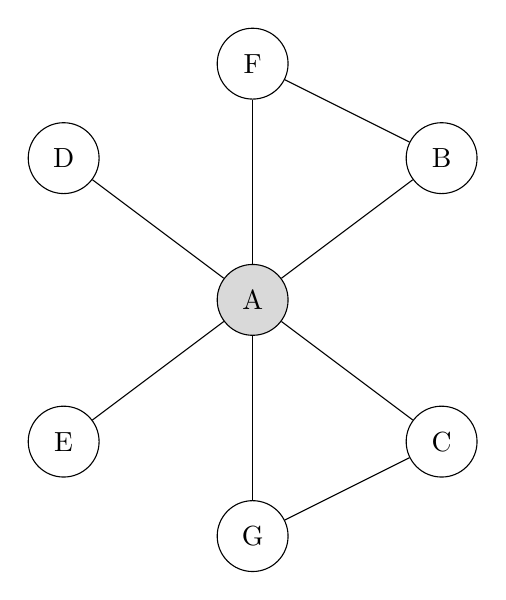
\begin{tikzpicture}[scale=1.2, every node/.style={circle, draw, minimum size=0.9cm}]
% Hubs
\node[fill=gray!30] (A) at (0,0) {A};
\node (B) at (2,1.5) {B};
\node (C) at (2,-1.5) {C};
\node (D) at (-2,1.5) {D};
\node (E) at (-2,-1.5) {E};
\node (F) at (0,2.5) {F};
\node (G) at (0,-2.5) {G};

\draw (A) -- (B);
\draw (A) -- (C);
\draw (A) -- (D);
\draw (A) -- (E);
\draw (A) -- (F);
\draw (A) -- (G);
\draw (B) -- (F);
\draw (C) -- (G);
\end{tikzpicture}
\end{center}

En este grafo, el nodo A es un hub: tiene muchas más conexiones que el resto, lo cual es característico del modelo.

Las redes libres de escala representan una clase fundamental de redes complejas que se encuentran en numerosos sistemas naturales y artificiales. El modelo de Barabási–Albert provee una base simple para modelar este tipo de estructuras. En el análisis de arquitecturas neuronales y el diseño de algoritmos de aprendizaje automático sobre grafos, este modelo resulta esencial.